\documentclass[../main.tex]
		
		\begin{document}
			\section{Vertex Degrees}
	\begin{description}
		\item[Task:] Use numbers to understand incidence relationships.
		\item[Definition:] Let $(V, E)$ be a graph. The \underline{degree} deg $v$ of a vertex $v \in V$ is defined as the number of edges of the graph that are incidence to $v$, \textbf{i.e.} the number of edge with $v$ as one of their endpoints.
		\item[Example:] ~\\
		\begin{figure}[h!]
			\centering
			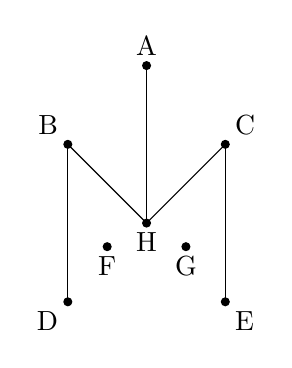
\begin{tikzpicture}
			\coordinate (A) at (0, 0);
			\coordinate (H) at (0, -2);
			\coordinate (B) at (-1, -1);
			\coordinate (C) at (1, -1);
			\coordinate (D) at (-1, -3);
			\coordinate (E) at (1, -3);
			\coordinate (F) at (-0.5, -2.3);
			\coordinate (G) at (0.5, -2.3);
			
			\draw (A) -- (H);
			\draw (H) -- (B);
			\draw (H) -- (C);
			\draw (B) -- (D);
			\draw (C) -- (E);
			
			\draw[fill=black] (A) circle[radius=0.5mm] node[above]{A};
			\draw[fill=black] (B) circle[radius=0.5mm] node[above left]{B};
			\draw[fill=black] (C) circle[radius=0.5mm] node[above right]{C};
			\draw[fill=black] (D) circle[radius=0.5mm] node[below left]{D};
			\draw[fill=black] (E) circle[radius=0.5mm] node[below right]{E};
			\draw[fill=black] (H) circle[radius=0.5mm] node[below]{H};
			\draw[fill=black] (F) circle[radius=0.5mm] node[below]{F};
			\draw[fill=black] (G) circle[radius=0.5mm] node[below]{G};
			\end{tikzpicture}
		\end{figure}
		~\\
		def $f$ = deg $g$ = 0 \\
		deg $d$ = deg $e$ = deg $a$ = 1 \\
		deg $b$ = deg $c$ = 2 \\
		deg $h$ = 3 \\
		\item[Definition:] A vertex of degree 0 is called an \underline{isolated} vertex.
		\item[Definition:] A vertex of degree 1 is called a \underline{pendent} vertex.
		\item[Theorem:] Let $(V, E)$ be a graph. Then $\sum_{v \in V}$deg $v = 2\#(E)$, where $\sum_{v \in V}$deg $v$ is the sum of the degrees of all the vertices of the graph, and $\#(E)$ is the number of edges of the graph.
		\item[Proof:] $\sum_{v \in V}$deg $v$ is the sum of all the entries in the adjacency matrix. Every edge $vv' \in E$ contributes 2 to the sum $\sum_{v \in V}$deg $v$, 1 for the vertex $v$ and 1 for the vertex $v' \Rightarrow$ each edge must be counted twice, so $\sum_{v \in V}$deg $v = 2 \#(E)$.
		\item[qed]
		\item[Corollary:] $\sum_{v \in V}$deg $v$ is an even integer.
		\item[Proof:] Since $\sum_{v \in V}$deg $v = 2 \#(E)$, and $\#(E) \in \mathbb{N}$, the result follows.
		\item[qed]
		\item[Corollary:] In any graph, the number of vertices of odd degrees must be even.
		\item[Proof:] Assume not, then $\sum_{v \in V}$deg $v$ is an odd integer as $odd + even = odd \Rightarrow \Leftarrow$ to the previous corollary.
		\item[qed]
		\item[Definition:] A graph is called k-regular for some non-negative integer $k$ if every vertex of the graph has degree equal to $k$.
		\item[Example:] A rectangle is 2-regular. \\
		\begin{figure}[h!]
			\centering
			\begin{tikzpicture}
				\coordinate (A) at (0, 0);
				\coordinate (B) at (4, 0);
				\coordinate (D) at (0, -2);
				\coordinate (C) at (4, -2);
				
				\draw (A) node[above left]{A} -- (B);
				\draw (A) -- (D) node[below left]{D};
				\draw (B) node[above right]{B} -- (C);
				\draw (D) -- (C) node[below right]{C};
			\end{tikzpicture}
		\end{figure}
		deg $a$ = deg $b$ = deg $c$ = deg $d$ = 2.
		\item[Definition:] A graph $(V, E)$ is called \underline{regular} is $\exists k \in \mathbb{N}$ s.t. $(V, E)$ is k-regular.
		\item[Corollary:] Let $(V, E)$ be a k-regular graph. Then $k\#(V) = 2\#(E)$ where $\#(V)$ is the number of vertices and $\#(E)$ is the number of edges.
		\item[Proof:] By the theorem, $\sum_{v \in V}$deg $v = 2\#(E)$, but $(V, E)$ is k-regular $\Rightarrow$ deg $v = k \forall v \in V$. Therefore $\sum_{v \in V}$deg $v = \#(V).k = 2 \#(E)$.
		\item[qed]
		\item[Example:] Consider a complete graph $(V, E)$ with $n$ vertices. $(V, E)$ is $(n-1)$-regular because every vertex is adjacent to all the remaining $(n-1)$ vertices.
		\item[Corollary:] A complete bipartite graph $k_{p,q}$ is regular $\Leftrightarrow p = q$
		\item[Proof:] Recall that $V=V_1 \cup V_2 \hspace{10mm} V_1 \cap V_2 = \emptyset$ for a bipartite graph. \\
		$\Leftarrow$ is $p=q, \forall v \in V_1$ satisfies that deg $v = p = q$ and $\forall v \in V_2$ satisfies that def $v=p=q$ since the graph is complete $\Rightarrow (V, E)$ is p-regular. \\
		$\Rightarrow \: (V, E)$ is regular $\Rightarrow \forall v \in V_1$ and $\forall v' \in V_2$, deg $v=$ deg $v'$, but $(V, E)$ is complete $\Rightarrow v$ is adjacent to all vertices in $V_2$, \textbf{i.e.} def $v = \#(V_1)$ and $v'$ is adjacent to all vertices in $V_1$, \textbf{i.e.} deg $v' = \#(V_2) \rightarrow \#(V_1) = \#(V_2)$
	\end{description}
	

\end{document}